\section{Lines in $\R^3$}

\begin{boxdefinition}[Joint]
    A \textbf{joint} in $\R^3$ is an intersection point of $3$ non-coplanar lines.
\end{boxdefinition}

In other words, any point at which three lines that do not share a plane in common meet is called a joint.

We ask ourselves the following question: how many joints can a collection of $L$ lines have?

Let's denote the greatest such number $J(L)$.

Here's one construction: just an $n \times n \times n$ grid. This gives you $3n^2$ lines and $n^3$ joints.

\begin{figure}[H]
    \centering
    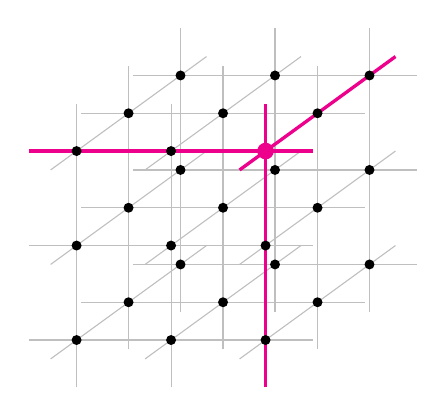
\begin{tikzpicture}[x = {(1cm, 0cm)}, y = {(0.55cm, 0.4cm)}, z = {(0cm, 1cm)}, scale = 1.2]
        \foreach \a in {0, 1, 2}{
            \foreach \b in {0, 1, 2}{
                \draw[gray!50] (-0.5, \a, \b) -- (2.5, \a, \b);
                \draw[gray!50] (\a, -0.5, \b) -- (\a, 2.5, \b);
                \draw[gray!50] (\a, \b, -0.5) -- (\a, \b, 2.5);
            }
        }
        \draw[very thick, magenta] (-0.5, 0, 2) -- (2.5, 0, 2);
        \draw[very thick, magenta] (2, -0.5, 2) -- (2, 2.5, 2);
        \draw[very thick, magenta] (2, 0, -0.5) -- (2, 0, 2.5);
        \foreach \a in {0, 1, 2}{
            \foreach \b in {0, 1, 2}{
                \foreach \c in {0, 1, 2}{
                    \fill[black] (\a, \b, \c) circle (1.5pt);
                }
            }
        }
        \fill[magenta] (2, 0, 2) circle (2.5pt);
    \end{tikzpicture}
\end{figure}
The case $n = 3$ is drawn above, with the three lines through one of the joints highlighted. Every point of the grid is a joint, and every line of the grid is parallel to one of the axes and passes through $n$ of them.

\begin{boxlemma}
    In any collection of lines with $J$ joints, some line is in $\leq 3J^{\frac{1}{3}}$ joints.
\end{boxlemma}
\begin{proof}
    \sorry
\end{proof}

Assuming the lemma, we notice that
\begin{align*}
    J(L)
    &\leq J(L - 1) + 3J(L)^{\frac{1}{3}} \\
    &\leq J(L - 2) + 3 \cdot 2 \cdot J(L)^{\frac{1}{3}} \\
    &\leq J(L - 3) \cdots \\
    &\leq 3 \cdot L \cdot J(L)^{\frac{1}{3}}
\end{align*}
The first inequality comes from taking $L$ lines with $J(L)$ joints and deleting a line that, by the lemma, is in at most $3J(L)^{\frac{1}{3}}$ of them. Every other joint is still a joint of the remaining $L - 1$ lines, so $J(L) - 3J(L)^{\frac{1}{3}} \leq J(L - 1)$. The same argument gives $J(L - 1) \leq J(L - 2) + 3J(L - 1)^{\frac{1}{3}}$, and $J(L - 1) \leq J(L)$, since adding a line to a collection destroys none of its joints; this is the second line. Carrying on down to $J(0) = 0$, each of the $L$ lines we delete costs at most $3J(L)^{\frac{1}{3}}$ joints, which is the last line. Dividing it by $J(L)^{\frac{1}{3}}$ gives $J(L)^{\frac{2}{3}} \leq 3L$, ie,
\begin{align*}
    J(L) \leq \parenth{3L}^{\frac{3}{2}} = \BigO{L^{\frac{3}{2}}}
\end{align*}
So the grid is optimal up to a constant factor: it has $L = 3n^2$ lines and $n^3 = \parenth{\frac{L}{3}}^{\frac{3}{2}}$ joints.

Let's now take a detour into the world of polynomials.

Our notation for this course isn't amazing. Let $\F$ be a field.

\begin{boxnotation}
    $\poly_D\of{\F^n}$ denotes the set
    \begin{align*}
        \setst{p \in \F\!\brac{x_1, \ldots, x_n}}{\deg_{\tot}\of{p} \leq D}
    \end{align*}
    where $\deg_{\tot}$ denotes the total degree of the polynomial.
\end{boxnotation}

The monomials form a basis of this space. By a stars and bars argument, we can show that the number of monomials is $\binom{D + n}{n}$. So this is the dimension of this space.

% [CORRECTED] was: "$\abs{S} \leq \dim\of{\poly_D\of{\F^n}}$, there is some $p$", and "the inequality $\abs{S} \leq \parenth{\text{dimension of space}}$" below --- $p = 0$ always vanishes, and at equality the kernel can be $0$ (eg, $n = 1$ and $D + 1$ distinct points), so the inequality has to be strict
Observe the following: if $S \ssq \F^n$ is such that $\abs{S} < \dim\of{\poly_D\of{\F^n}}$, there is some nonzero $p \in \poly_D\of{\F^n}$ that vanishes on $S$. The proof is simple: consider the evaluation map
\begin{align*}
    \ev : \poly_D\of{\F^n} \to \F^{S} : p \mapsto \parenth{p(s)}_{s \in S}
\end{align*}
Rank-nullity\footnote{Tarun would be so proud!} and the inequality $\abs{S} < \parenth{\text{dimension of space}}$ tells us the dimension of the kernel is positive, which gives us some $p$ as desired.
